%!TEX root = Thesis_David_Burns.tex
\chapter{Modelling}
\label{ch:model}

The complexity of the atmosphere and the processes within it, detailed in \cref{ch:atmo}, require modelling to produce theoretical descriptions of the systems. Generally, a number of models are chained together to simulate different parts of the climate system. Each of these models is built upon a number of theories that are used depending on the state of the system at the time \citep[Chapter 21]{jacobson2005fundamentals}. This complexity makes atmospheric modelling difficult and broad. Fortunately many models have been developed around the world to fill niches such as \gls{hysplit} for trajectory modelling, the Unified Model for climate and weather modelling and \gls{ccam} for atmospheric modelling \citep{draxler:1997tga, mann:2010wb, cope:2009tz, mcgregor2008updated}.

The first choice to make when deciding which model to use is between a Global Climate Model (\gls{gcm}) and a Regional Climate Model (\gls{rcm}). The difference is in the granularity achieved in the discretisation used to solve the governing equations, and the requirements of boundary conditions \citep{thatcher:2015wy}. A \gls{rcm} is run on a smaller scale for a specific region with a high density of grid points. As only a small portion of the Earth's surface is simulated, the values of parameters at the boundary of that region must be known in advance \citep{hurley2002air}. Usually these boundary conditions are obtained from a previous run of a \gls{gcm}. Although a \gls{gcm} is less restrictive than a \gls{rcm}, its lack of high resolution may miss small but critical details. Conversely, the regional restriction of a \gls{rcm} can miss distant events that may influence the climate in the simulated region \citep[Chapter 25]{seinfeld2012atmospheric}.

% 'one short paragraph on this'
% What are the base equations most models use?
% Reduced versions of the navier stokes eqns...
% What ways can we numerically solve these equations?
% finite difference
% finite element
% operator splitting
% finite volume?
% 'include a sentence from this in the above paragraph to illustrate approximations'
% Obviously the full blown navier stokes equations are far too complicated to solve. So what approximations are generally used by climate modellers to still encapsulate some of the more complicated flow dynamics?
% An example is eddy diffusivity. Eddy currents occur on both small and large scales and are the result of turbulent flow around obstacles such as land masses 'cite'. A constant called the eddy diffusivity attempts to cover mixing due to eddy currents. I think this is a good example of the limitations in atmospheric models and attempts to use simple equations to approximate more complex phenomena.
% Actually it seems like most models neglect normal diffusion in favour of turbulent diffusion as the rate of turbulent diffusion dominates regular diffusion \citep[Chapter 17]{seinfeld2012atmospheric}.


% Whats the difference between eulerian and lagrangian modelling?
% What is semi-lagrangian modelling? benefits?


% what is sensitivity to initial conditons and what effect does this have on models?
% How can we tell when models are accurate?
% What methods should we use to decide if the model is good? (this is before data is taken so i mean things like sensitivity analysis), cite examples of things like sensitivity analysis, switching various things on and off to understand what is happening.


%--------------------------------------------------------------------------------------------------------------------------%
%--------------------------------------------------------------------------------------------------------------------------%

	\section{Back Trajectory Modelling}
	\label{sec:backtraj}

	When working in atmospheric science, it is often necessary to model the trajectories that parcels of air travel. With the advent of large scale meteorological measurements, the data required to model this process is now being produced. Trajectory modelling is able to take a particular location and predict, forward or backward in time, the path a parcel of air travels to or from that location. It can be used to predict whether air at a particular location has passed over a region or event of interest or, for example, whether there has been contamination from anthropogenic sources \citep{draxler:1998vr}. \gls{hysplit} is one such trajectory model. \gls{hysplit}'s efficacy in performing back trajectory modelling is well established \citep{draxler:1998vr}. It has been used to model many different scenarios from forecasting fire smoke movement \citep{rolph:2010in} to nuclear cloud dispersion \citep{rolph:2014kk}.

%--------------------------------------------------------------------------------------------------------------------------%
%--------------------------------------------------------------------------------------------------------------------------%

	% \section{Unified Model}
	% \label{sec:unimod}
	% 'contemplate dumping this paragraph'

	% The Unified Model (\gls{um}) is a suite of models produced by the United Kingdom Met Office. One of the submodels for dealing with chemistry and aerosols is the United Kingdom Chemistry \& Aerosols model \gls{ukca}. One of the aerosol sub models for \gls{ukca} is \gls{glomapm}. This is a version of a combined meteorological, chemical, and aerosol model with feedback throughout the submodels 'site some unified model description paper'.

%--------------------------------------------------------------------------------------------------------------------------%
%--------------------------------------------------------------------------------------------------------------------------%

	\section{CCAM, CTM, GLOMAP}
	\label{sec:ccg}

	For modelling the full aerosol pathway, from atmospheric, to chemical transport, to aerosol microphysics CSIRO uses a trio of models: \gls{ccam}, \gls{ctm} and \gls{glomapm}. This combination of models has been used previously in the Sydney Particle Study \citep{cope:2014tw}. The Sydney Particle Study was a large scale study performed by seven different organisations and lead by CSIRO. It encompassed both measurement and modelling of fine particles in the Sydney area, with a view to understand their exposure to Sydney's population. Both \gls{ccam} and \gls{tapm} (an alternative meteorological model produced by \gls{csiro}) were used as the \gls{rcm}s for the study. Their outputs were compared with each other, and with the collected data. \gls{ctm}, and consequently \gls{glomapm}, were used for the particle dynamics and chemical transport modelling within the two \gls{rcm}s. Both \gls{rcm}s performed well, with predictions of sea salt, organic matter and secondary inorganic aerosols within \SI{15}{\percent} of observations (see \cref{fig:sydpartdata}) \citep{cope:2014tw}.

	\begin{figure}[!htb]
	    \centering
	    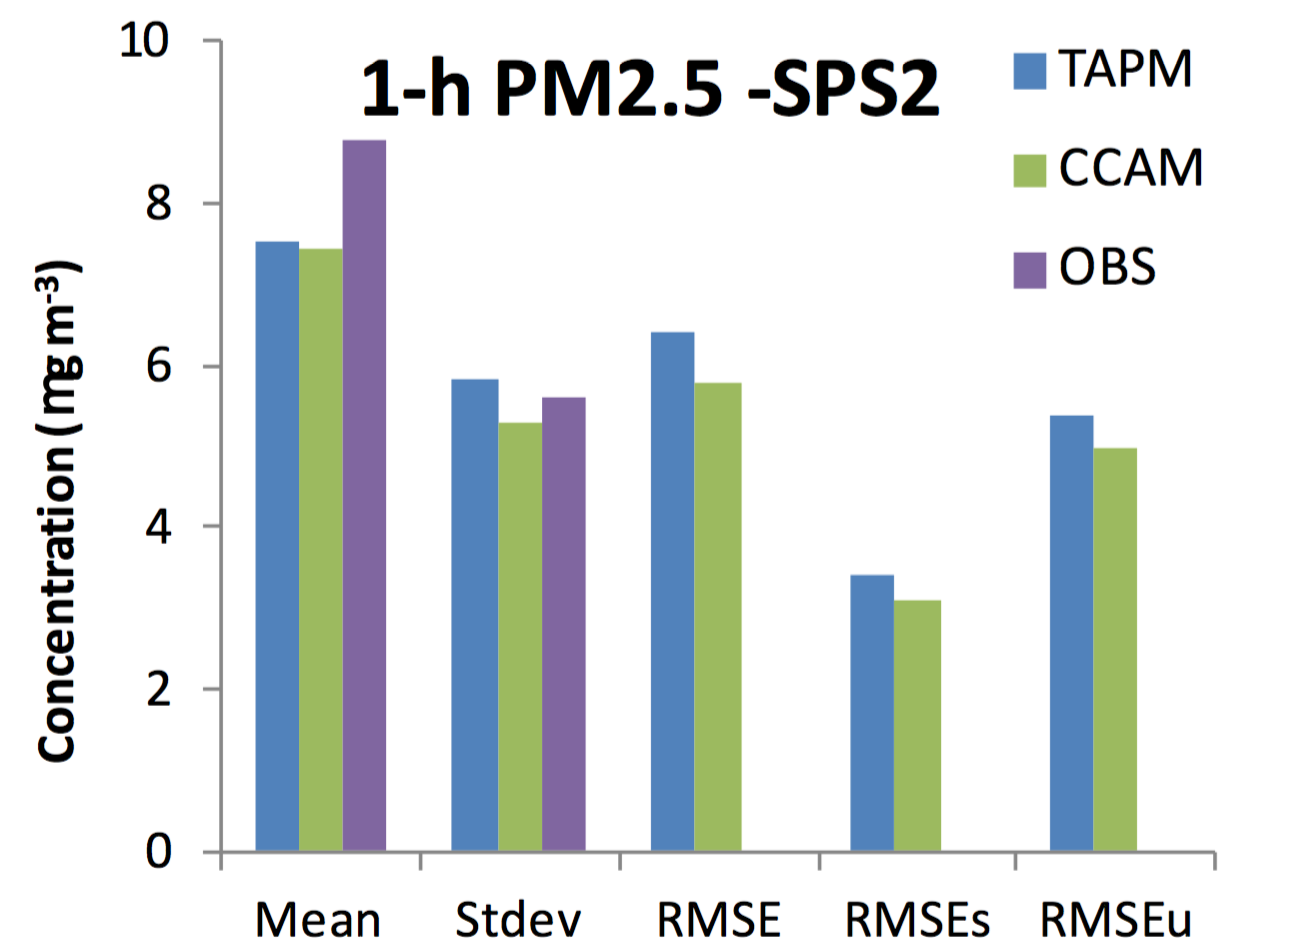
\includegraphics[width=0.6\textwidth,natwidth=1308,natheight=952]{Fig/Literature_Review/sydneyparticledata.png}
	    \caption{The hourly averaged concentrations of $\mathrm{PM}_{2.5}$ particles for the second Sydney Particle Study. Both \gls{ccam} and \gls{tapm} used as the base meteorological model produce similar average concentrations, close to observation \citep{cope:2014tw}.}
	    \label{fig:sydpartdata}
	\end{figure}
